\chapter{Approach}
\label{cha:approach}
In this chapter, we describe the approach of this thesis by presenting the main ideas to reach our goals for the simulation and high-level agent in section~\ref{sec:goals_and_approaches}. In section~\ref{sec:architecture}, we present the architectural approach.

\section{Goals and Approaches}
\label{sec:goals_and_approaches}
\textbf{Realistic simulation:} An important goal of the thesis is a high realism of the simulation. The realism can be defined by the similarity of sensor data and consequences of robot actions between simulation and reality. A more realistic simulation allows more compete testing because more real problems can be simulated. The realism of the simulation has many different aspects. The first group of aspects is about the realism of sensor data. There are some sensors that are easy to simulate, such as distance sensors, bumpers and gyroscopes. Others, especially cameras, are more difficult to simulate realistically. The choice of Gazebo with ODE and Ogre for the visual appearance already allows us to simulate a wide range of sensors realistically. Also the noise in the sensor data is important for the realism of the simulation. For all metric sensors, we simulate this as Gaussian noise with the calculated value as mean and a configurable variance. The second group of aspects are about the realism of the physical environment. Objects have to behave in the simulation and the reality in a similar way. This is especially important for robot movement and manipulation tasks. Here, Gazebo with ODE also provides high realism out of the box. Nevertheless, it is important to find good physical parameters for the simulated objects. Examples of those parameters are the mass and coefficients of friction. Another important aspect of simulation-realism is that the simulation should not introduce new problems which do not occur in reality. Such a problem, which occurred in the development of the thesis, is that the simulation ran slower than the system time but the robot software used the system time. This caused to early triggering of timeouts. We solve this problem by providing the simulation time in Fawkes.\\
\textbf{Different levels of simulation:} Sometimes, it is also useful to test with a more abstract and less realistic simulation. This allows testing the optimal case without sensor noise or without using low level components, such as localization, if those produce new errors or are not finished yet. To be able to simulate on different levels, we use the multi-level abstraction approach~\cite{MultiLevelAbstraction} presented in the chapter~\ref{cha:related_work}. We use multi-level abstraction for sensing and for actuators. How we use multiple abstraction levels is shown in the next section about the architecture.\\
\textbf{Compatibility with original robot software:} We want to achieve that the robot software runs in the same way in the simulation as in reality. This is important because otherwise it would result in additional effort to keep the robot software running in the simulation. This effort can also cause more difference between simulation and reality. In the thesis, the simulation components should provide the same interfaces as the real components that are simulated. In Fawkes, this is easy to achieve because the interfaces between components are well defined and components using an interface do not recognize whether the interface is provided by the simulation or a real component.\\
\textbf{Efficient testing:} We want to make the use of the simulation as efficient as possible. To achieve this, we provide scripts which automatically start the full simulation with all needed programs. Without these scripts, it would take much more time. For a full simulation of an LLSF game, it is necessary to start Gazebo, the Refbox, a controlling Fawkes instance and, for the Robotinos, three times Fawkes, \texttt{roscore} and \texttt{move\_base}. Each program-instance has to be started with correct parameters.  Another approach we use to increase the efficiency is the feature to load different configurations and setups. For example, the scripts are able to load the simulation with different numbers of Robotinos, abstraction levels and simulation environments. Loading different configurations for the robot software is a feature of Fawkes and useful for us. We also integrated this into the scripts. Furthermore, we provide the possibility to draw objects into the simulation. This makes it possible to visualize belief and intention of a robot to identify mistakes or ways to improve the system~\cite{Visualization}.\\
\textbf{Multi-robot system evaluation:} An important part of this thesis is the evaluation of multi-robot systems. Here, the features we already mentioned in the previous paragraph are especially useful because the testing effort (e.g. to setup the simulation or analyzing the coordination between robots) often scales with the number of robots. To evaluate the performance of the multi-robot system faster without having to observe the simulation all the time, we provide the possibility to run multiple simulation runs, in our case runs of LLSF games, automatically. With this feature, the simulation can run, for example, 20 times over night. To analyze executed simulation runs, we keep statistics of each run. For our LLSF domain, we keep the amount of achieved points with a detailed list of all actions that provided points with the time. These statistics can easily be extended by the amount of collisions between robots, waiting time for resource locks or other useful measurements. Sometimes, it can happen that single simulation runs have a very different results. To find the reason for this result, we keep log files of each run and also record the simulation itself. With this record, the simulation run can be reconstructed. The record contains the position and movements of all objects in the simulation. Here, it is also useful to draw additional information, such as the localization of the robots, in the simulation to be able to analyze faults without having to look in the log files. Automated simulation runs also allow the comparison of different configurations of the multi-robot system. The automation script can be started with a number of configurations to test. This can be useful for finding the best performing role combination or parameters such as thresholds.\\
\textbf{Expandability and flexibility:} An essential criterion of a good simulation is the expandability to adapt to future changes. On the one hand, there will be changes to the Carologistics Robotino and to the LLSF. These changes have to be easy to implement in the simulation, otherwise the simulation would not remain useful. On the other hand, it is attractive to use the simulation also in other domains, such as RoboCup@Home. To achieve the expandability of the simulation, we provide a framework for simulated devices in Gazebo and Fawkes. Furthermore, we focus on developing small modules that are exchangeable and reusable. In Gazebo, new modules can easily be added to robot and world plugins. In Fawkes, it is easy to implement a new plugin which provides the wanted features because the plugin can use the provided Gazebo aspect. The simulation should also be flexible to adapt to small changes. Therefore, we provide several configuration files for the simulation environment, for the simulated objects and robots and for plugins in Gazebo and Fawkes.\\
\textbf{Agent improvements:} It is easy to see that the current approach we showed in section~\ref{sec:multi_agent_strategies} has limitations which obstruct a significantly better performance of our multi-robot system. The static role approach does neither allow a tighter cooperation between the agents nor that the agent behavior can take the situation into account. For example, if there is not enough time to produce another $P_1$ or $P_2$ puck or there are no more $P_1$ or $P_2$ pucks ordered, the $P_1P_2$ role would still start another production. Therefore, we want to introduce a dynamic role change to switch roles in specified situations. Furthermore, we want to introduce recycling because it can lead to simple points and provides an alternative possibility to get new $S_0$ pucks. A third way to improve the performance of our system is to make use of three robots instead of just two.\\


\section{Architecture}
\label{sec:architecture}

\subsection{Simulation}
\label{sec:architecture_simulation}
\begin{figure}
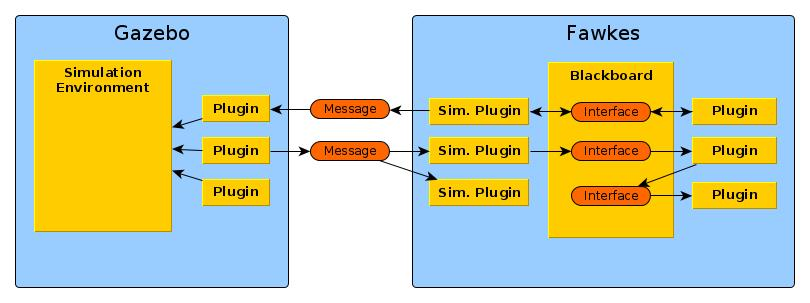
\includegraphics[width=\textwidth]{tabs/fawkes_gazebo}
\caption{Architecture of the simulation}
\label{fig:fawkes_gazebo}
\end{figure}
The basic structure of the simulation is shown in Figure~\ref{fig:fawkes_gazebo}. On the right side, there is the Fawkes robot software framework we want to run in the simulation. On the left side, there is the simulator Gazebo. Roughly, the simulation is composed of a simulation environment, which handles the physical and visual simulation of the environment with all included objects, and plugins associated to the world and all models with some kind of behavior. There are plugin instances for the sensors and actuators of each robot as well as plugins that control the world. At this point, Fawkes can be seen as a composition of plugins, which are used on the real robot system, simulation plugins, which communicate with the simulation and exchange original sensor and actuator plugins, and the blackboard. The blackboard manages several interfaces which are used for communication between Fawkes plugins. The Fawkes simulation-plugins send actuator messages to the corresponding Gazebo plugins and receive messages from sensor-plugins in Gazebo. This architecture has the advantage that it is flexible and extendable. To add a new sensor or actuator to the simulation, it is sufficient to create or modify a Gazebo plugin and a Fawkes simulation-plugin to provide the corresponding interface. Furthermore, the architecture is flexible enough to allow multi-level abstraction as we see later in this section. It is also easy to change plugins on either side. It is even possible to use the Gazebo simulation with another robot operating system than Fawkes. The other system just has to send and receive the same messages as our simulation-plugins.


\subsection{Communication Fawkes-Gazebo}
\label{sec:architecture_communication}
\begin{figure}
\center
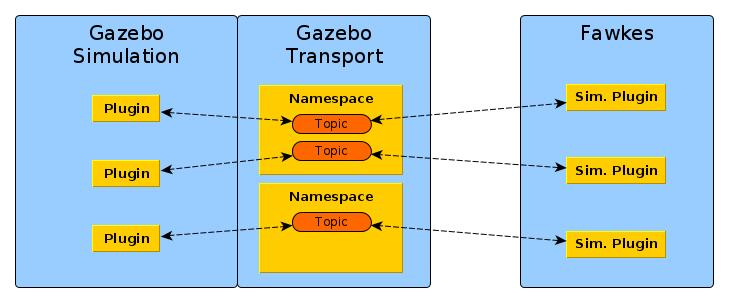
\includegraphics[width=\textwidth]{tabs/communication}
\caption{Communication between Fawkes and Gazebo}
\label{fig:communication}
\end{figure}
The communication between Fawkes and the Gazebo simulation has a specific structure to organize the distinction between multiple robots and different sensors and actuators. Figure~\ref{fig:communication} shows this structure. Fawkes simulation-plugins and Gazebo plugins communicate over a message-transport system. In our case, this system is embedded in the Gazebo Transport API. In the message-transport system, there are different namespaces which act as communication channels. There is one namespace for each simulated robot and for the simulated world. The topics in a namespace represent what the messages that are sent on this topic are about. Each plugin can listen to or send on the topics in a namespace. For example, there are topics about laser data and motor commands. This architecture is extendable because it is easy to add new namespaces or topics. It is flexible, because the communication through a topic in a namespace is a many-to-many relationship, and it is comfortable because instances of plugins in different Fawkes instances can listen to the same topic and get data from different simulated robots because the plugins listen do different channels.


\subsection{Multi-level Abstraction}
\label{sec:architecture_mla}
\begin{figure}
  \centering
  \begin{subfigure}[b]{\textwidth}
    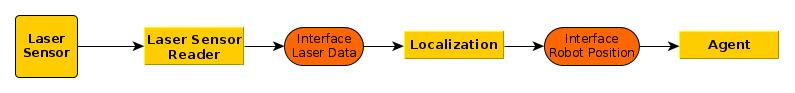
\includegraphics[width=\textwidth]{tabs/mla_hardware}
    \caption{With real hardware}
    \label{fig:mla_hardware}
  \end{subfigure}
  \begin{subfigure}[b]{\textwidth}
    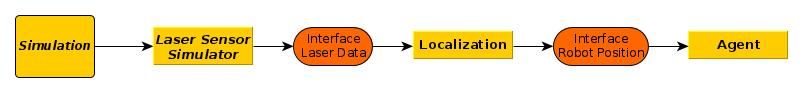
\includegraphics[width=\textwidth]{tabs/mla_sim_low}
    \caption{With low level abstraction}
    \label{fig:mla_sim_low}
  \end{subfigure}
  \begin{subfigure}[b]{\textwidth}
    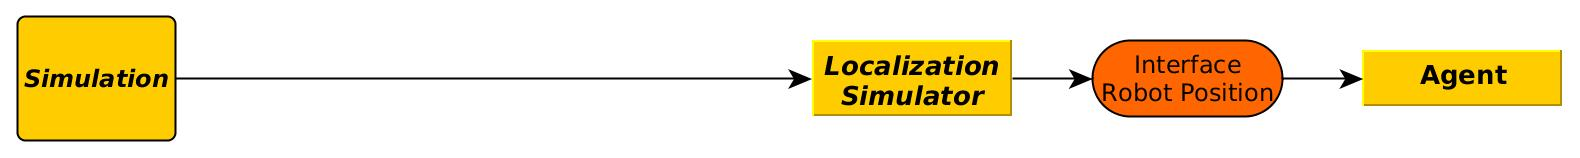
\includegraphics[width=\textwidth]{tabs/mla_sim_high}
    \caption{With high level abstraction}
    \label{fig:mla_sim_high}
  \end{subfigure}
  \caption[Example for multi-level abstraction]{Example for multi-level abstraction (The arrows indicate data flow.)}
  \label{fig:mla}
  
\end{figure}
Figure~\ref{fig:mla} shows how multi-level abstraction fits into our simulation architecture. We choose a simple example about the localization with laser data. Figure~\ref{fig:mla_hardware} shows the system as it is used in the real application. There is the laser sensor hardware, a plugin which reads out the sensor and publishes the laser data in an blackboard-interface, a localization plugin which uses the laser data interface to determine a robot position and to provide the position in another interface. Then, the robot agent uses the position information from the interface. Figure~\ref{fig:mla_sim_low} shows the system in the simulation with low level abstraction. The hardware is replaced by the simulation and the laser sensor reader by a simulation-plugin which receives the laser data from the simulation. This simulation-plugin provides the same interface as the original plugin. Another possibility with high level abstraction is shown in Figure~\ref{fig:mla_sim_high}. Here, the localization plugin is replaced by a simulation-plugin which simply looks up the position of the robot in the simulation and writes it in the interface. The agent can now be simulated with ground-truth position data without using of the original localization plugin. An example for multi-level abstraction for actuators could be the movement of a robot. It is possible to simulate the motors with motor commands from an interface or the motion of the robot by applying the motion command in an interface directly to the simulated robot.
